\documentclass[%
master,         % тип документа
%natbib,         % использовать пакет natbib для "сжатия" цитирований
subf,           % использовать пакет subcaption для вложенной нумерации рисунков
href,           % использовать пакет hyperref для создания гиперссылок
colorlinks=false % цветные гиперссылки
%,fixint=false  % отключить прямые знаки интегралов
%,times         % шрифт Times как основной
]{disser}

\usepackage[
  a4paper, mag=1000,
  left=2.5cm, right=1.5cm, top=2cm, bottom=2cm, headsep=0.7cm, footskip=1cm
]{geometry}
\usepackage[T2A]{fontenc}
\usepackage[utf8]{inputenc}
\usepackage[english,russian]{babel}
%\usepackage{tabularx,longtable}
\ifpdf\usepackage{epstopdf}\fi

\usepackage{algorithm}
\usepackage{algpseudocode}
\renewcommand{\listalgorithmname}{Список алгоритмов}
\floatname{algorithm}{Алгоритм \textnumero\hspace{-3pt}}

% Номера страниц снизу и по центру
\pagestyle{footcenter}
\chapterpagestyle{footcenter}

% Точка с запятой в качестве разделителя между номерами цитирований
%\setcitestyle{semicolon}

% Использовать полужирное начертание для векторов
\let\avec\vec
\renewcommand{\vec}[1]{\boldsymbol{\mathbf{#1}}}

\addto\captionsrussian{\renewcommand\chaptername{}}
\addto\captionsrussian{\renewcommand\thechapterfont{\Large\bfseries}}
\addto\captionsrussian{\renewcommand\tocprethechapter{}}
\addto\captionsrussian{\renewcommand\prethechapter{}}
\addto\captionsrussian{\renewcommand\postthechapter{.}}

\renewcommand{\studentlabel}{Выполнила студентка гр. 971}

% Включать подсекции в оглавление
\setcounter{tocdepth}{1}

\graphicspath{{fig/}}

\begin{document}

% Переопределение стандартных заголовков
\def\contentsname{Содержание}
\def\conclusionname{Выводы}
\def\bibname{Список использованных источников}

\institution{Министерство образования и науки Российской Федерации
\\
Федеральное государственное автономное образовательное учреждение\\[-6pt] высшего профессионального образования\\[-6pt]
«Московский физико-технический институт\\[-6pt]
(государственный университет)»
\\
ФАКУЛЬТЕТ УПРАВЛЕНИЯ И ПРИКЛАДНОЙ МАТЕМАТИКИ\\[-6pt]
КАФЕДРА ВЫЧИСЛИТЕЛЬНОЙ МАТЕМАТИКИ
\\
(Специализация «Прикладные вычислительные модели\\[-6pt] и программные комплексы»)}

% Имя лица, допускающего к защите (зав. кафедрой)
\apname{{Холодов А.С}}

\title{Выпускная квалификационная работа\\[-6pt](магистерская диссертация)}

\topic{Маршевый метод решения задачи переноса излучения}

% Автор
\author       {Павлова Екатерина Сергеевна} % ФИО
\group        {971} % Группа
\coursenum    {03.04.01} % Номер направления
\course       {Прикладные математика и физика}
\masterprognum{\phantom{.}010991\phantom{.}} % Номер магистерской программы
\masterprog   {Прикладные вычислительные модели \\\hspace{16.7em} и программные комплексы}

% Научный руководитель
\sa      {Скалько Юрий Иванович}
\sastatus{к.ф.-м.н.}
% Второй научный руководитель
%\sasnd      {ФИО руководителя}
%\sasndstatus{д.~ф.-м.~н., ст.~н.~с.}

% Рецензент
\rev      {Колдоба Александр Васильевич}
\revstatus{д.~ф.-м.~н.}

% Город и год
\city{Москва}
\date{\number\year}

\maketitle

% Содержание
\tableofcontents
% Введение
\intro
С необходимостью учитывать процессы излучения часто сталкиваются при численном моделирования высокотемпературных процессов. Среди них задачи, связанные с моделированием звездных атмосфер и межзвездного вещества, динамикой высокотемпературной плазмы, проектированием теплозащиты спускаемых аппаратов. Современные постановки этих задач существенно сложны и опираются, как правило, на трехмерное пространственное описание процессов. В то же время, в этих задачах излучение может иметь значительную и, даже, определяющую роль.

Сама по себе задача нахождения поля излучения довольно сложна. В общем случае, интенсивность излучения является функцией координат, времени, направления и частоты излучения. Решение полной задачи — крайне трудоемкая задача. Но влияние излучения на другие процессы обычно описывается некоторыми интегральными характеристиками интенсивности излучения. Поэтому, на практике, вместо полной постановки используется некоторым способом осредненная (по частотам, направлениям) приближенная постановка, имеющая существенно меньшую размерность.

Развитие численных методов для решения уравнения переноса излучения проходило с 50-х годов прошлого столетия. В то время разрабатывались методы, учитывающие ту или иную симметрию задачи, сводящую ее к эффективно одномерной или двумерной. Однако, эти методы совершенно непригодны для современных задач, и не являются универсальными.
% Глава 1
\chapter{Постановка задачи}

\section{Математическая модель}
Поле излучения, заполняющего пространство, описывается распределением интенсивности излучения по частотам, в пространстве и по направлениям переноса лучистой энергии. Пусть $f(\nu, \vec r, \vec \Omega, t)d\nu d\vec r d \vec \Omega \, $ есть число световых квантов в спектральном интервале от $ \nu$ до $ \nu + d\nu$, находящихся в момент $t$ в элементе объема $d\vec r$ около точки $\vec r$ и имеющих направление движения в элементе телесного угла $d\vec \Omega$ около единичного вектора $\vec \Omega$. 
Каждый квант обладает энергией $h \nu$ и движется со скоростью $c$, поэтому величина 
\begin {equation}
I_{\nu} (\vec r, \vec \Omega, t)d \nu d\vec \Omega = h\nu c f (\nu, \vec r, \vec \Omega, t)d\nu d\vec{\Omega}
\end {equation}
есть количество лучистой энергии в спектральном интервале $d\nu$, протекающей в $1 \text{ сек}$ через площадку в $1 \text{ см}^2$, помещенную в точке $\vec r$ перпендикулярно к направлениям распространения энергии, которые лежат в элементе телесного угла $d\vec\Omega$ около вектора $\vec \Omega$. Задание функций $I_{\nu}$ или $f$ полностью определяет поле излучения. Количество лучистой энергии, заключенной  спектральном интервале $d\nu$ и находящейся в $1 \text{ см}^3$ пространства в точке $\vec r$ в момент $t$, или спектральная плотность излучения, равно:
\begin {equation}
U_\nu (\vec r, t) = h \nu \int_{4 \pi} f d \Omega = \frac{1}{c} \int_{4\pi} I_{\nu} d\Omega.
\end {equation}

Вектор спектрального потока равен 
\begin {equation}
\vec S_{\nu} = \int I_{\nu}\vec\Omega d\Omega,
\end {equation}
где $\vec\Omega$ - единичный вектор направления движения квантов. 
Полные интенсивность, плотность и поток излучения получаются из спектральных интегрированием их по всему спектру частот:
\begin {equation}
I = \int_0^\infty I_{\nu} d\nu, \quad U = \int_0^\infty U_{\nu}d\nu, \quad \vec S =  \int_0^\infty \vec S_{\nu}d\nu.
\end {equation}
\section{Уравнение переноса}
Рассмотрим баланс излучения в элементарном цилиндре \ref{fig:1} с площадью основания $d\sigma$ и высотой $ds$, расположенном в данной точке пространства таким образом, что направление $\vec\Omega$ совпадает с образующей цилиндра и перпендикулярно к его основаниям. За время $dt$ в левое основание втекает количество излучения $I_{\nu} (\vec\Omega, \vec r,t)d\sigma dt$. Из правого основания за тот же промежуток времени вытекает количество излучения $(I_{\nu} + dI_{\nu})d \sigma dt$.

\begin{figure}[bh]
\centering{
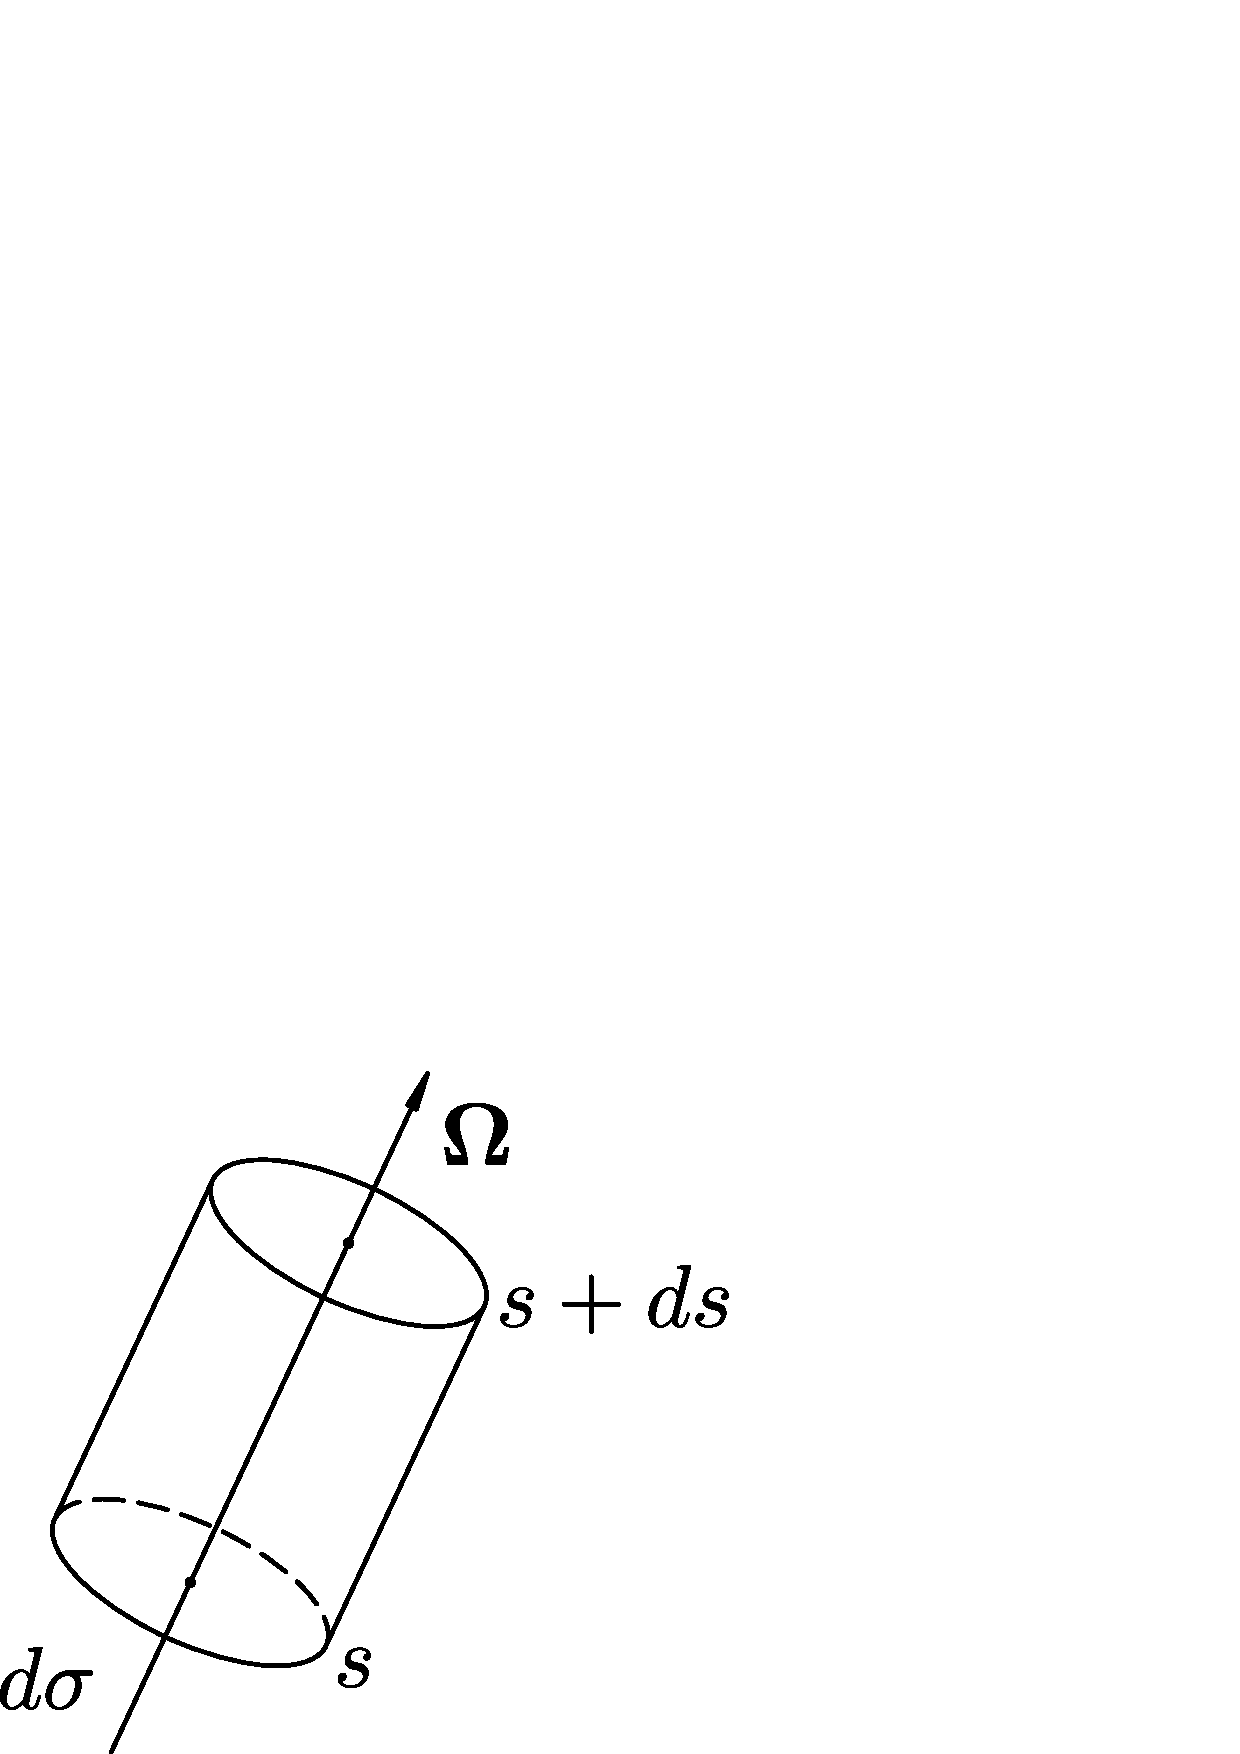
\includegraphics[width = 0.5\textwidth]{cylinder.png}
}
\caption{К выводу уравнения переноса излучения}
\label{fig:1}
\end{figure}

Интенсивность $I_{\nu}$ есть функция координат и времени. Приращение интенсивности пучка света при переходе от левого основания к правому складывается из локального приращения за время прохождения светом пути $ds$ и из приращения при переходе от координаты $s$ к координате $s+ds$ в данный момент времени, 
\begin {equation}
dI_{\nu}  = \frac{\partial I_{\nu}}{\partial t } \frac{ds}{c}+\frac{\partial I_{\nu}}{\partial s}ds.
\end {equation}

Введем коэффициент поглощения $\varkappa_\nu$ таким образом, что количество лучистой энергии в интервале частот $d\nu$ и интервале направлений $d\vec\Omega$, поглощаемой в $1 \text{ см}^3$ в  $1 \text{ сек}$, равно
\begin {equation}
I_{\nu}d\nu d\vec\Omega \varkappa_{\nu}.
\label {3}
\end {equation}
Обозначим плотность самопроизвольного испускания $j_\nu$. То есть количество энергии, самопроизвольно испускаемой веществом  в $1 \text{ см}^3$ в  $1 \text{ сек}$ интервале $d\nu d\vec\Omega$, равно $j_{\nu}d\nu d\vec\Omega$. Помимо самопроизвольного испускания также существует так называемое вынужденное испускание. Вероятность вынужденного испускания кванта данной частоты и данного направления пропорциональна имеющейся в данной точке пространства интенсивности излучения той же частоты и того же направления. Известно \cite{zeld_2013}, что полная вероятность испускания данных квантов пропорциональна величине $1+n$, где $n = c^2I_{\nu}/2h\nu^3$. Таким образом, полное количество излучения, испускаемого в $1 \text{ сек}$ в $1 \text{ см}^3$ в интервале $d\nu d\vec\Omega$, равно 
\begin {equation}
j_{\nu} d\nu d\vec\Omega \left(1+\frac{c^2}{2h\nu^3}I_{\nu}\right).
\label{4}
\end {equation}
Первое слагаемое в скобках соответствует спонтанному испусканию, а второе - вынужденному. 

Количество излучения, испущенного в цилиндре за время $dt$, согласно формуле \eqref{4}, равно
\begin {equation}
j_{\nu}\left(1 + \frac {c^2}{2h\nu^3}I_{\nu}\right)d\sigma ds dt.
\end {equation}
Поглощается в нем за то же время количество излучения $\varkappa_{\nu} I_{\nu}d\sigma dsdt$. Составляя баланс и поделив полученное выражение на произведение дифференциалов $d\sigma dsdt$, получим уравнение
\begin {equation}
\frac{1}{c} \left(\frac{\partial I_{\nu}}{\partial t} + c \vec \Omega \nabla I_{\nu}\right) = j_{\nu} \left(1 + \frac {c^2}{2h\nu^3}I_{\nu}\right) - \varkappa_{\nu}I_{\nu}.
\label{1}
\end {equation}

Преобразуем правую часть уравнения \eqref{1}, объединив вместе члены, отвечающие поглощению и вынужденному испусканию, поскольку они оба пропорциональны неизвестной функции координат и времени - интенсивности излучения. 

Рассмотрим среду, находящуюся в состоянии термодинамического равновесия при постоянной температуре $T$. В стационарных условиях поле излучения также равновесно. Спектральная функция плотности равновесного излучения $U_{\nu p}$ подчиняется закону Планка. Количество энергии равновесного излучения частоты $\nu$ в $1 \text{ см}^3$, приходящееся на единичный интервал частот, равно
\begin {equation}
U_{\nu p} = \frac{8 \pi h \nu^3}{c^3} \frac {1}{e^{\frac{h\nu}{kT}} - 1}
\end {equation}
В силу изотропии спектральная интенсивность равновесного излучения равна
\begin {equation}
I_{\nu p} = \frac{cU_{\nu p}}{4\pi} = \frac{2h\nu^3}{c^2}\frac{1}{e^{\frac{h\nu}{kT}} - 1}
\label{5}
\end {equation}

В состоянии термодинамического равновесия испускание и поглощение квантов данных частоты и направления в точности компенсируют друг друга, так что выражения \eqref{3} и \eqref{4} следует приравнять, причем интенсивность излучения $I_{\nu}$ заменить при этом равновесной величиной $I_{\nu p}$. 
Принимая во внимание формулу \eqref{5} для равновесной интенсивности, найдем, что отношение лучеиспускательной способности любого вещества к его коэффициенту поглощения есть универсальная функция частоты и температуры:
\begin {equation}
\frac{j_{\nu}}{\varkappa_{\nu}} =  \frac{I_{\nu p}}{1+\frac{c^2}{2h\nu^3}I_{\nu p}} = \frac{2h\nu^3}{c^2}e^{-\frac{h\nu}{kT}}.
\label{6}
\end {equation}

Это отношение представляет собой одну из форм закона Кирхгофа. Формулу \eqref{6} удобно переписать в виде
\begin {equation}
j_{\nu} = I_{\nu p}\varkappa_{\nu}\left(1-e^{-\frac{h\nu}{kT}}\right).
\label{7}
\end {equation}

В новой трактовке закон Кирхгофа \eqref{7} приобретает форму
\begin {equation}
j_{\nu} = \varkappa'_{\nu}I_{\nu p}, \quad \varkappa'_{\nu} = \varkappa_{\nu}\left(1 - e^{-\frac{h\nu}{kT}}\right).
\end {equation}

Введем при этом в множитель перед $I_{\nu}$ в члене вынужденного испускания вместо коэффициента излучения $j_{\nu}$ его выражение через коэффициент поглощения, в которое подставим формулу \eqref{5} для равновесной интенсивности. Правая часть уравнения \eqref{1} примет вид 
\begin {equation}
j_{\nu} - \varkappa_{\nu}\left(1 - e^{-\frac{h\nu}{kT}}\right)I_{\nu}.
\end {equation}
Отсюда видно, что вынужденное испускание можно трактовать как некое уменьшение поглощения: часть квантов поглощается и тут же испускается снова с той же частотой и в том же направлении, причем вероятность этого <<переизлучения>> равна $e^{-\frac{h\nu}{kT}}$. Можно считать, что коэффициент поглощения имеет несколько меньшую величину:
\begin {equation}
\varkappa'_{\nu} = \varkappa_{\nu}\left(1 - e^{-\frac{h\nu}{kT}}\right).
\end {equation}

Взаимодействие излучения с веществом можно представлять так, как будто существует только спонтанное испускание и эффективное поглощение, описываемое коэффициентом $\varkappa'_{\nu}$, исправленным на вынужденное испускание. 

Вводя это выражение в правую часть уравнения переноса \eqref{1} запишем уравнение в следующей форме:
\begin {equation}
\frac{1}{c}\frac{\partial I_{\nu}}{\partial t} + (\vec\Omega \nabla) I_{\nu} = \varkappa'_{\nu} (I_{\nu p} - I_{\nu}).
\label{2}
\end {equation}

Будем в дальнейшем понимать под $\varkappa_\nu$ коэффициент поглощения $\varkappa_\nu'$, т.е. подправленный на спонтанное излучение.
\section {Граничные условия}
Дополним уравнение \eqref{2} граничными условиями. Они должны определять только излучение, приходящее извне в исследуемый объем. Мы ограничиваемся случаем заданного излучения извне, поскольку условия отражения связывают уравнения переноса в разных направлениях. В случае выпуклых областей для направлений $\vec\Omega$, выходящих в рассматриваемую область, имеет место неравенство $(\vec\Omega, \vec n) < 0$, где $\vec n$ -- вектор внешней нормали к границе $\Gamma$ (см рис \ref{fig:6}).
\begin{figure}[ht!]
	\centering{
		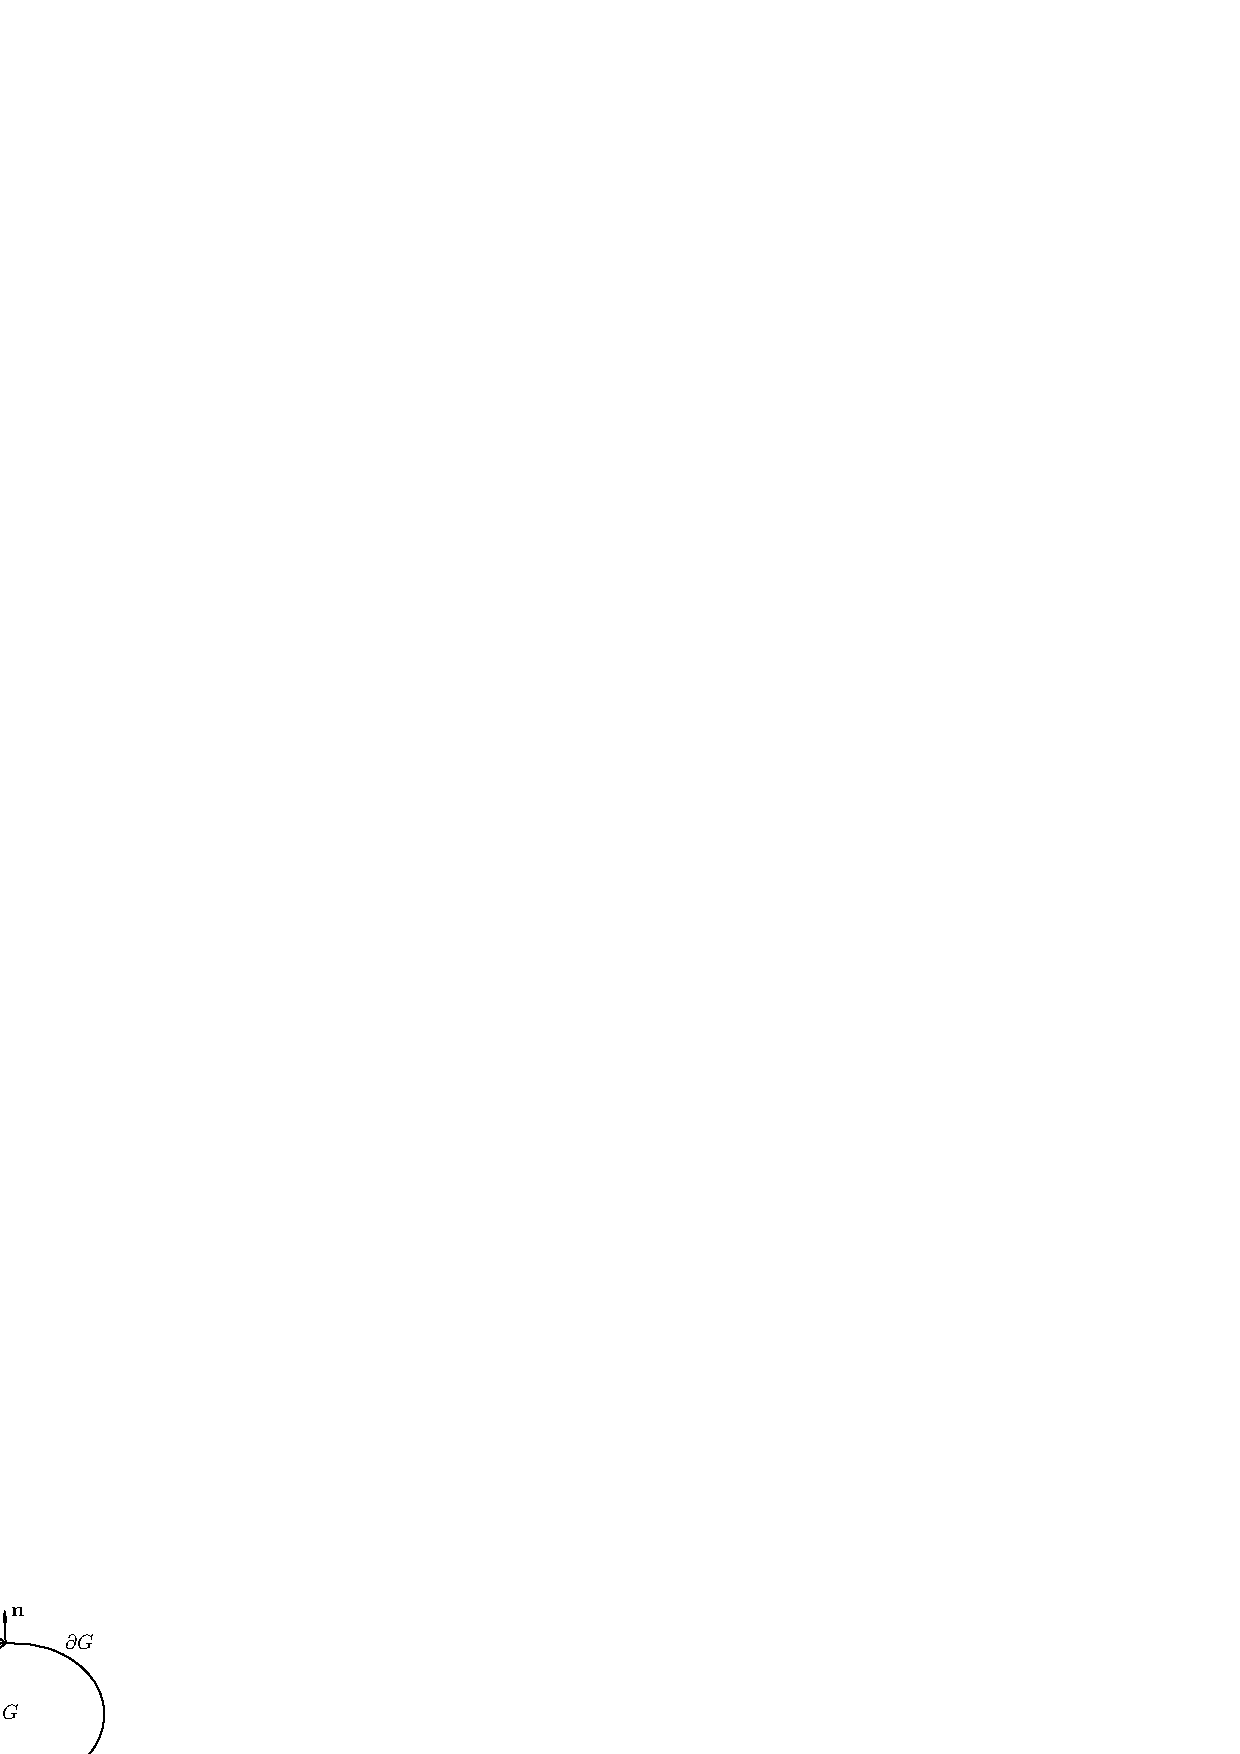
\includegraphics[width = 0.5\textwidth]{bord.png}
	}
	\caption{Граничные условия для выпуклых областей. На участке границы $\Gamma_1$ происходит зеркальное отражение фотонов.}
	\label{fig:6}
\end{figure}

Граничное условие на $\Gamma$ примет вид
\begin {equation}
I_\nu (\Gamma, \vec\Omega, \nu, t) = I_\nu^*(\Gamma, \vec\Omega, \nu, t), \quad (\vec\Omega, \vec n) < 0.
\end {equation}
Здесь $I_\nu^*$ - известная функция, определяющая приходящее извне излучение. В работе используется граничное условие вида
\begin {equation}
I_\nu (\Gamma, \vec\Omega, \nu, t) = 0, \quad (\vec\Omega, \vec n) < 0.
\end {equation}
Это условие соответствует тому, что источники излучения находятся только внутри рассматриваемой области.
Иногда часть границы области $\Gamma_1$ отражает выходящее из объема излучение. Простейшим случаем отражения является зеркальное отражение. При этом отражение происходит по законам классической оптики:
\begin {equation}
I_\nu (\Gamma, \vec\Omega, \nu, t) = \delta I_\nu(\Gamma_1, \vec\Omega_1, \nu, t), 
\end {equation}
где $\vec\Omega_1$ - симметричное к $\vec\Omega$ относительно нормали направление, $\delta$ - коэффициент отражения, $0 \leqslant \delta \leqslant 1$.
\section{Аналитическое решение уравнения переноса}
Найдем формальное решение уравнения переноса излучения, рассматривая величины, зависящие только от состояния вещества $I_{\nu p}(T)$, $\varkappa_{\nu}(T, \rho)$, как известные функции координат и времени. Рассмотрим сначала для простоты стационарный случай, когда распределения температуры и плотности, а также поле излучения не зависят от времени. Будем интересоваться излучением в точке $\vec r$ тела с направлением распространения $\vec \Omega$ \ref{fig:2}. 
\begin{figure}[ht!]
\centering{
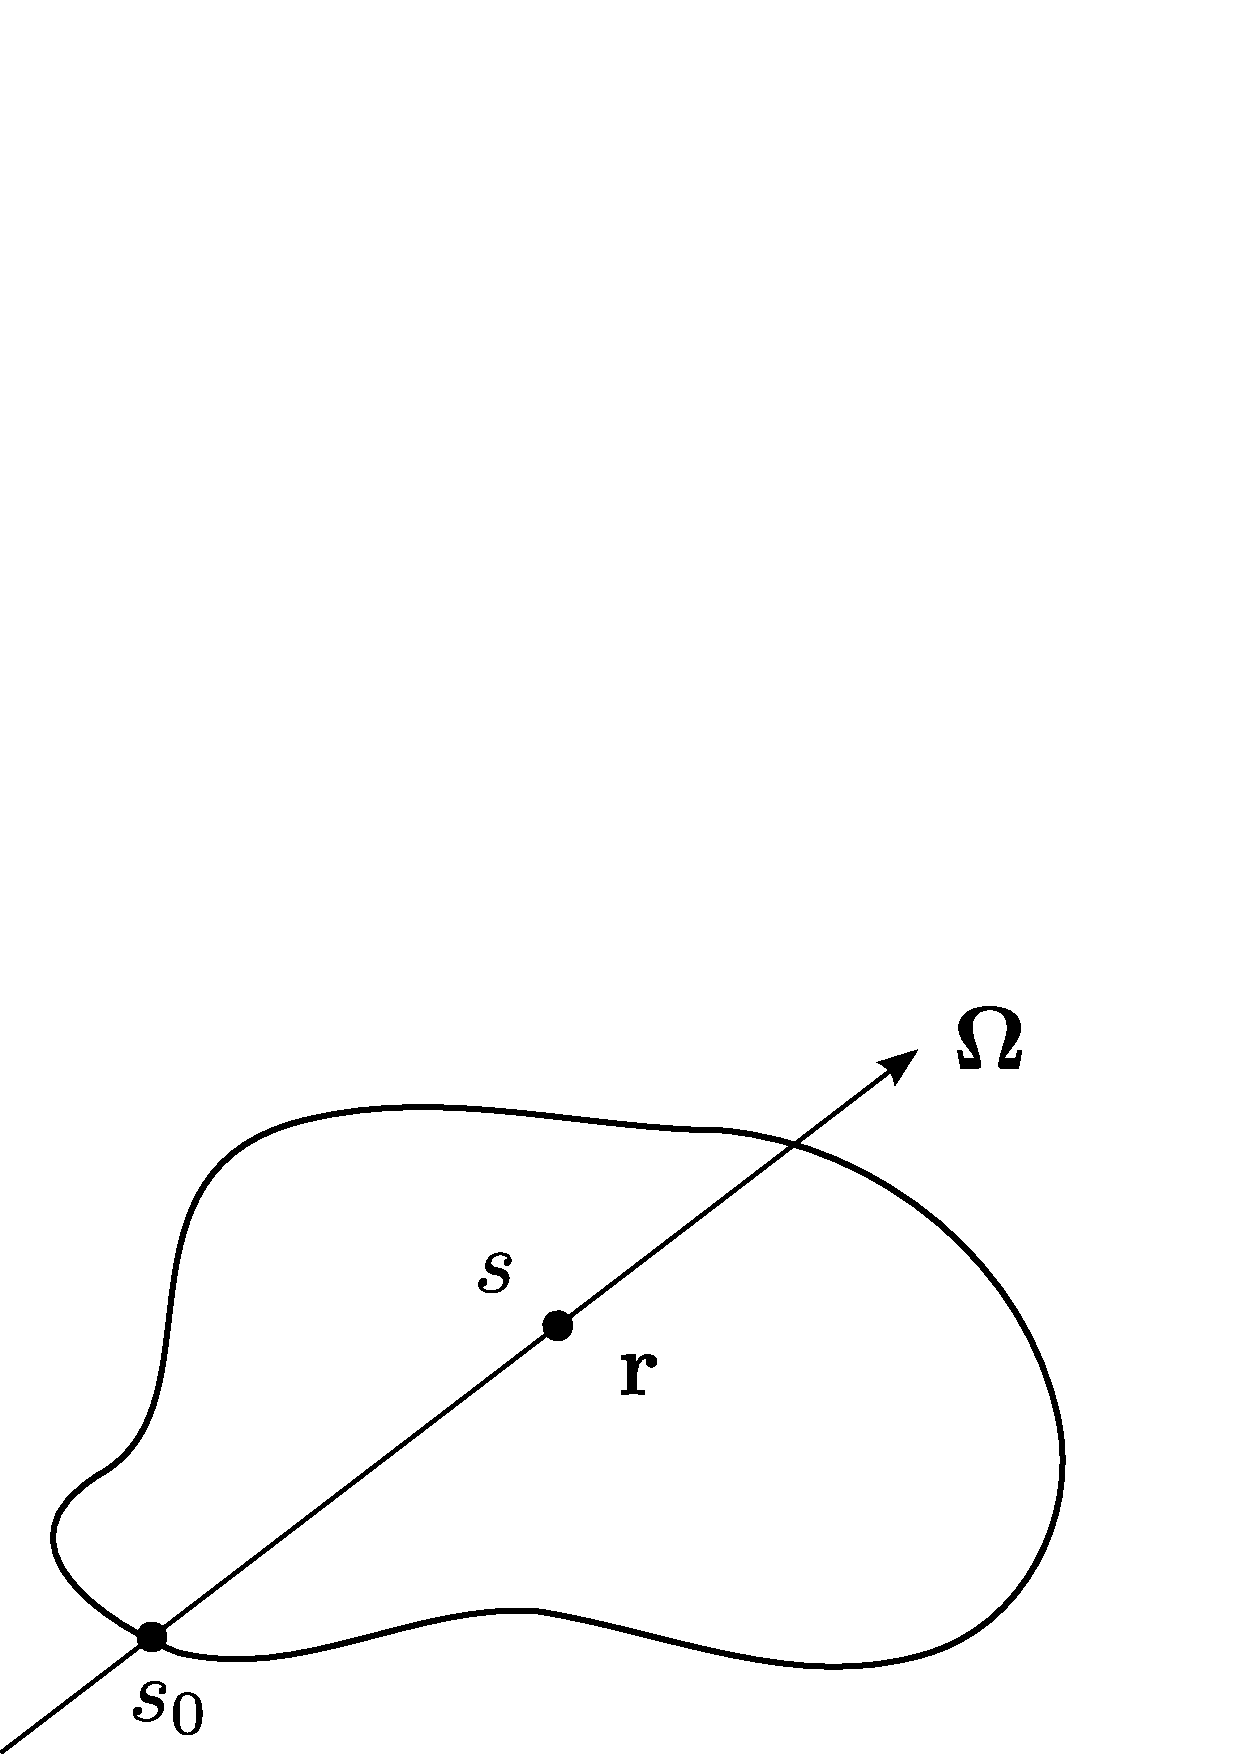
\includegraphics[width = 0.5\textwidth]{analytic.png}
}
\caption{Схема, поясняющая пределы интегрирования в формуле \eqref{8}}
\label{fig:2}
\end{figure}
Проведем луч через данную точку в данном направлении и обозначим координату вдоль луча через $s$. Замечая, что дифференциальное выражение в левой части уравнения переноса \eqref{2} представляет собой полную производную от интенсивности вдоль луча распространения, перепишем уравнение в виде
\begin {equation}
\frac{dI_{\nu}}{ds} + \varkappa_{\nu}I_{\nu} = \varkappa_{\nu}I_{\nu p}.
\end {equation}
Это уравнение можно рассматривать как обыкновенное линейное уравнение относительно интенсивности вдоль луча. Решение его есть:
\begin {equation}
I_{\nu}(s) = \int_{s_0}^s\varkappa_{\nu}I_{\nu p} \exp\Big[-\int_{s'}^s\varkappa_{\nu}ds''\Big]ds' + I_{\nu,0} \exp\Big[-\int_{s_0}^s \varkappa_{\nu}ds''\Big].
\label{8}
\end {equation}

Здесь $I_{\nu}(s)$ - интенсивность $I_{\nu}(\vec r, \vec\Omega)$, которая рассматривается как функция координаты $s$ вдоль луча. Интегрирование по лучу ведется от границы тела $s_0$ (как показано на \ref{fig:2}). Через $I_{\nu, 0}$ обозначена константа интегрирования, которая имеет смысл значения интенсивности излучения на границе в точке $s_0$.


% Глава 2
\chapter{Численный метод}

Численный метод. Выбирается фиксированный набор направлений. В этих направлениях решается уравнение переноса. Решение строится маршевым методом (за один проход по области, нет итераций). Интегральные характеристики излучения (плотность и поток излучения) рассчитываются по квадратурной формуле, согласованной с набором направлений. Для решения задачи в одном направлении используется метод, использующий короткие характеристики. Все грани тетраэдров делятся на входящие и
выходящие. На выходящих гранях берется несколько точек, из которых выпускаются характеристики до пересечения с входными гранями. Вдоль каждой короткой характеристики решение строится по формуле 
\begin {equation}
I = I^*e^{\varkappa \lambda)} + I_p (1 - e^{-\varkappa \lambda})
\end {equation}
Постоянное значение решения на грани. Необходимо выпустить 1 характеристику. Линейное распределение решения на грани. Необходимо выпустить 3 характеристики

\section{Общие положения метода коротких характеристик}
\section{Подробное описание метода коротких характеристик (входные/выходные грани...)}
\section{Маршевый метод (упорядочивание, Делоне, алгоритм для не-Делоне)}
Для того, чтобы посчитать решение на выходящих гранях, нужно упорядочить тетраэдры. Это возможно, если нет циклов. В сетках, удовлетворяющих условию Делоне, циклов гарантированно нет. Упорядочивание тетраэдров производится алгоритмом окрашивания, аналогичным поиску в ширину. Используется очередь тетраэдров, в которую тетраэдр попадает при окрашивании одной из входящих граней, а удаляется, когда все его входящие грани окрашены.
\section{Особенности выбора точек на грани (случай 1D, когда схема не устойчива)}
В одномерном случае на равномерной сетке видны проблемы, если узлы брать строго внутри граней. При малых числах Куранта характеристики остаются в пределах того же элемента, и численное решение не сходится к точному (численное решение меняется только в одной ячейке, в то время как точное должно переноситься) На неструктурированной сетке этот эффект не проявляется, но, возможно, снижает порядок метода.
\section{Повышение порядка пространственной аппроксимации. Монотонная интерполяция}
Для метода первого порядка узлы взяты в вершинах граней. Решение на грани является линейной функцией координат. Схема всегда монотонна

Для метода второго порядка узлы взяты в вершинах и на ребрах. Решение на грани является квадратичной функцией координат. Схема немонотонна, чтобы обеспечить монотонность нужно использовать ограничитель. Для обеспечения монотонности достаточно, чтобы квадратичная интерполяция на каждом ребре была монотонной Квадратичная интерполяция по трем точкам будет монотонной, если выполнено соотношение (). Если соотношение нарушается, значение в центре корректируется
% Глава 3
\chapter{Результаты}

\section{Сравнение методов первого и второго порядка}
\subsection{Решение уравнения в одном направлении}
Сравнение методов проводилось на следующей задаче. Рассматривалась
геометрическая область, куб со стороной $a = 2$. В центре области находится
крест, состоящий из пяти одинаковых кубиков со стороной $b = 0.2$ (см. рис. \ref{fig:6}).
\begin{figure}[ht!]
\centering{
\includegraphics[width = 0.5\textwidth]{cross.png}
}
\caption{Расчетная область}
\label{fig:6}
\end{figure}
Коэффи\-циент поглощения в области равен $\varkappa_1=0$, а внутри креста - $\varkappa_2 = 100$. Равновесная интенсивность в центральной области $1$, а в окружающей среде - $0$. Решение строилось вдоль одного направления, $\omega = (0,0,1)$ на сетке с $415625$ тетраэдрами и $76247$ вершинами. Изучалось решение на выходящей грани куба. 
\begin{figure}[ht!]
\centering{
\includegraphics[width = 0.3\textwidth]{1ord.png}%
\includegraphics[width = 0.3\textwidth]{2nolim.png}%
\includegraphics[width = 0.3\textwidth]{2wilim.png}
}
\caption{Сравнение решений методами первого порядка (слева), второго (в центре) и второго с ограничителем(справа).}
\label{fig:7}
\end{figure}

Точное решение должно представлять собой крест с интенсивностью $1 -
e^{b\varkappa_2} = 1-e^{-20} \approx 1$. Мы можем видеть (см. рис. \ref{fig:7}), что для первого порядка диффузия достаточно велика, второй порядок без ограничителя отклоняется от допустимых пределов $I \in [0, 1]$ на $20 \%$.
\subsection{Сравнение плотности излучения}
На той же самой задаче изучалась плотность излучения в центральном сечении куба, но коэффициенты поглощения изменились следующим образом: $\varkappa_1 = 10$, $\varkappa_2 = 1$. . Использовались 170 направлений из квадратурной формулы Лебедева \cite{lebedev_1999}. 

\begin{figure}[ht!]
\centering{
\includegraphics[width = \textwidth]{U2vs1.png}
}
\caption{Сравнение плотности излучения в центральном сечении куба. Слева второй порядок, справа --- первый.}
\label{fig:9}
\end{figure}

\begin{figure}[ht!]
\centering{
\includegraphics[width = \textwidth]{U2vs1Line.png}
}
\caption{Плотность излучения вдоль оси $Oz$. Красный второй порядок, синий - первый.}
\label{fig:10}
\end{figure}
Сравнение плотности излучения \ref{fig:9} и \ref{fig:10} показывает схожие результаты: интенсивность в центре куба в методе второго порядка на $\approx 2 \%$ больше, чем в случае метода первого порядка. В случае метода второго порядка \ref{fig:9} более выражен <<эффект луча>>, в то время как в методе первого порядка этот эффект сглажен за счет численной диффузии. 

\section{Сравнение методов первого и второго порядка с одинаковым количеством степеней свобод}
\section{Более сложная задача из астрофизики}


% Заключение
\conclusion
Построен маршевый вычислительный алгоритм для решения стационарной задачи переноса излучения на неструктурированной трехмерной сетке во многогрупповом приближении. В основе маршевого метода лежит алгоритм упорядочения тетраэдров. В данной работе построен более универсальный алгоритм упорядочения тетраэдров, чем описанный в \cite{skalko_2014}, так как работает для более широкого класса триангуляций, чем триангуляции, удовлетворяющие условию Делоне.

Было найдено необходимое условие устойчивости данного численного метода, применительно к модельной задаче на равномерной сетке. Был реализован метод второго порядка аппроксимации и его монотонная модификация. 

Проведено сравнение методов на различных модельных задачах. Показано, что немонотонный вариант метода второго порядка может иметь нефизические осцилляции величиной порядка $20 \%$. Продемонстрировано различное качественное поведение численной диффузии излучения для методов первого и второго порядков аппроксимации.

Вычислительный алгоритм был применен к прикладной задаче воспроизведения спектра излучения звезды по результатам МГД моделирования взаимодействия магнитного поля звезды с веществом аккреционного диска. 

% Список литературы
\bibliography{thesis}
\bibliographystyle{utf8gost71u}

% Приложения
\appendix
\chapter{Алгоритмы}

\begin{algorithm}[ht!]
\centering
\begin{algorithmic}[1]
\Function{ShiftToStable}{$e, Q$}
\State $\lambda := 1$
\State $\delta := \epsilon \cdot d(e)$
\State $\vec r_M := $ \Call{MassCenter}{$e$}
\For{каждой грани $f \in e$}
\State $(\vec r_i, \dots) := $ \Call{VertexCoordinates}{$f$}
\Comment Выбрать точку $\vec r_i \in f$
\State $\vec n_i := $ \Call{FaceNormal}{$f$}
\State $\vec r_{Q'} = \lambda \vec r_Q + (1 - \lambda) \vec r_{M}$
\If{$(\vec r_i - \vec r_{Q'}, \vec n_i) > \delta$}
\State \textbf{continue} \Comment Перейти к следующей грани
\Else
\State $\triangleright$ Найти точку пересечения отрезка $QM$ и плоскости
\State $\lambda := \frac{\delta - (\vec r_i - \vec r_M, \vec n_i)}
{(\vec r_Q - \vec r_M, \vec n_i)}$
\EndIf
\EndFor
\State $\vec r_{Q'} = \lambda \vec r_Q + (1 - \lambda) \vec r_{M}$
\State\Return{$Q'$}
\EndFunction
\end{algorithmic}
\caption{Пример алгоритма}
\label{alg:shift}
\end{algorithm}

\end{document}
